\section{Utility of Auxiliary Classifiers}

\cite{szegedy2015going} has introduced the notion of auxiliary classifiers
to improve the convergence of very deep networks. The original motivation was
to push useful gradients to the lower layers to make them immediately
useful and improve the convergence during training by combating the
vanishing gradient problem in very deep networks. Also Lee et al\cite{lee2014deeply}
argues that auxiliary classifiers promote more stable learning and better
convergence.
\begin{figure}
\centering
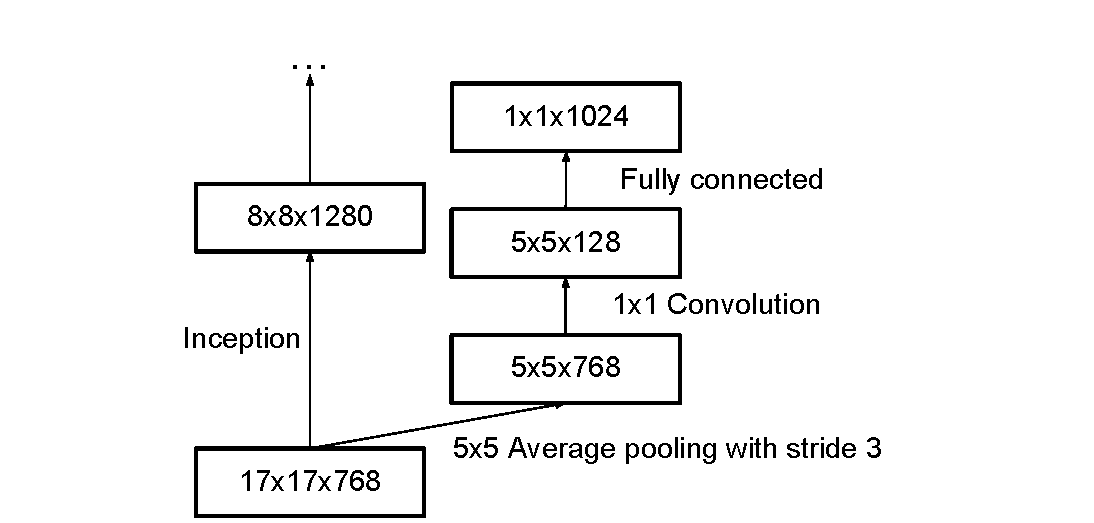
\includegraphics[width=\linewidth]{sideheaddiag.pdf}
\caption{Auxiliary classifier on top of the last $17\times 17$ layer.
Batch normalization\cite{ioffe2015batch} of the layers in the side head
results in a $0.4\%$ absolute gain in top-$1$ accuracy. The lower axis shows
the number of itertions performed, each with batch size $32$.}
\label{fig:sidehead}
\end{figure}
Interestingly, we found that auxiliary classifiers did not result in improved
convergence early in the training: the training progression of network with
and without side head looks virtually identical before both models reach
high accuracy. Near the end of training, 
the network with the auxiliary branches starts to
overtake the accuracy of the network without any auxiliary branch and
reaches a slightly higher plateau.

Also \cite{szegedy2015going} used two side-heads at different stages in the
network. The removal of the lower auxiliary branch did not have any
adverse effect on the final quality of the network. Together with the
earlier observation in the previous paragraph, this means that
original the hypothesis of \cite{szegedy2015going} that these branches
help evolving the low-level features is most likely misplaced.
Instead, we argue that the auxiliary classifiers act as regularizer.
This is supported by the fact that the main classifier of the
network  performs better if the side branch is batch-normalized~\cite{ioffe2015batch}
or has a dropout layer. This also gives a weak supporting evidence for the
conjecture that batch normalization acts as a regularizer.
